%!TEX root = ../../main.tex
%Khaled -> Model comparision
\chapter{Modeling}
\label{cha:Modelling}

%----------------------------------------------------------------------------------------
In this phase, we have successfully completed the data preparation phase and our five sliding windows are ready to use. \newline \newline
Modeling is an iterative process, in which we can apply several modeling techniques to the same problem using the default parameters and then fine-tune them until we satisfy our quality criteria. There is not a single model and a single execution which can satisfactorily answer our questions. For this, we tested several models to find the one that best fits our problem.\newline \newline
This phase comprises tasks such as select modeling techniques, generate test design, build model and assess model.


%----------------------------------------------------------------------------------------
\section{Select Modeling Techniques}

As a first step in modeling, we decided to choose Supervised Machine Learning algorithms, to perform multi-class classification because our objective is to predict the final result of a match between two teams, if there is a win by the home team, a draw or a win by the away team. \newline \newline
Therefore, we have selected Decision Trees and Neural Networks as techniques in order to test its performance and find the most appropriate for our project.

%----------------------------------------------------------------------------------------
\section{Generate Test Design}

This part refers to the generation of a procedure to test the model quality and validity needs, before building our models. \newline \newline
For some modeling techniques, we have divided our dataset into training and test sets, the model is built based on the training set, and its quality is estimated based on the test set, which represents 30\% of the dataset. \newline
We also took care to not shuffle the dataset as we need to keep the last 10 matches of the sliding windows dataset in the correct order. \newline 
For others, we only used 5\% for test set, a small amount because we wanted to keep as much data as possible for training and validation. The remaining 95\% are divided into 80\% training and 20\% validation datasets.\newline \newline
For training the models, we used automated stop as a strategy, after the training loss did not improve more than 0.0001 for 10 consecutive epochs or the model exceeds 1000 training epochs.\newline \newline
To evaluate the models, we used the accuracy results as criteria.


%----------------------------------------------------------------------------------------
\section{Build Models}

The aim of this part is to build several models before comparing the results.\newline
Most modeling techniques have a number of parameters that can be adjusted to control the modeling process.\newline \newline
For our Supervised Machine Learning Algorithms, we used scikit-learn API to build a Decision Tree and Multi-Layer Perceptron neural network. We also used the TensorFlow/Keras framework to build basic sequential neural networks.\newline \newline
The Decision Tree can be modified by adjusting the depth of the tree. For Neural Networks, we can change the number of hidden layers, the neurons per layer and other parameters.


\subsection{Decision Tree Classifier}

A decision tree is a simple classification representation that learns from the data with a set of if-then-else decision rules.\newline \newline
% \cite {DecisionTree: scikit-learn}. 
Using the decision tree algorithm, we start at the root of the tree and divide the data on the feature that results in the largest information gain. We can then repeat this procedure until the leaves are pure.\newline \newline
In our project, we set the depth of the tree to four.\newline
The Decision Tree Classifier achieved an accuracy of 52.95\% using the first sliding window option as a dataset, as shown in the following Figure.
\begin{figure}[H]
\begin{center}
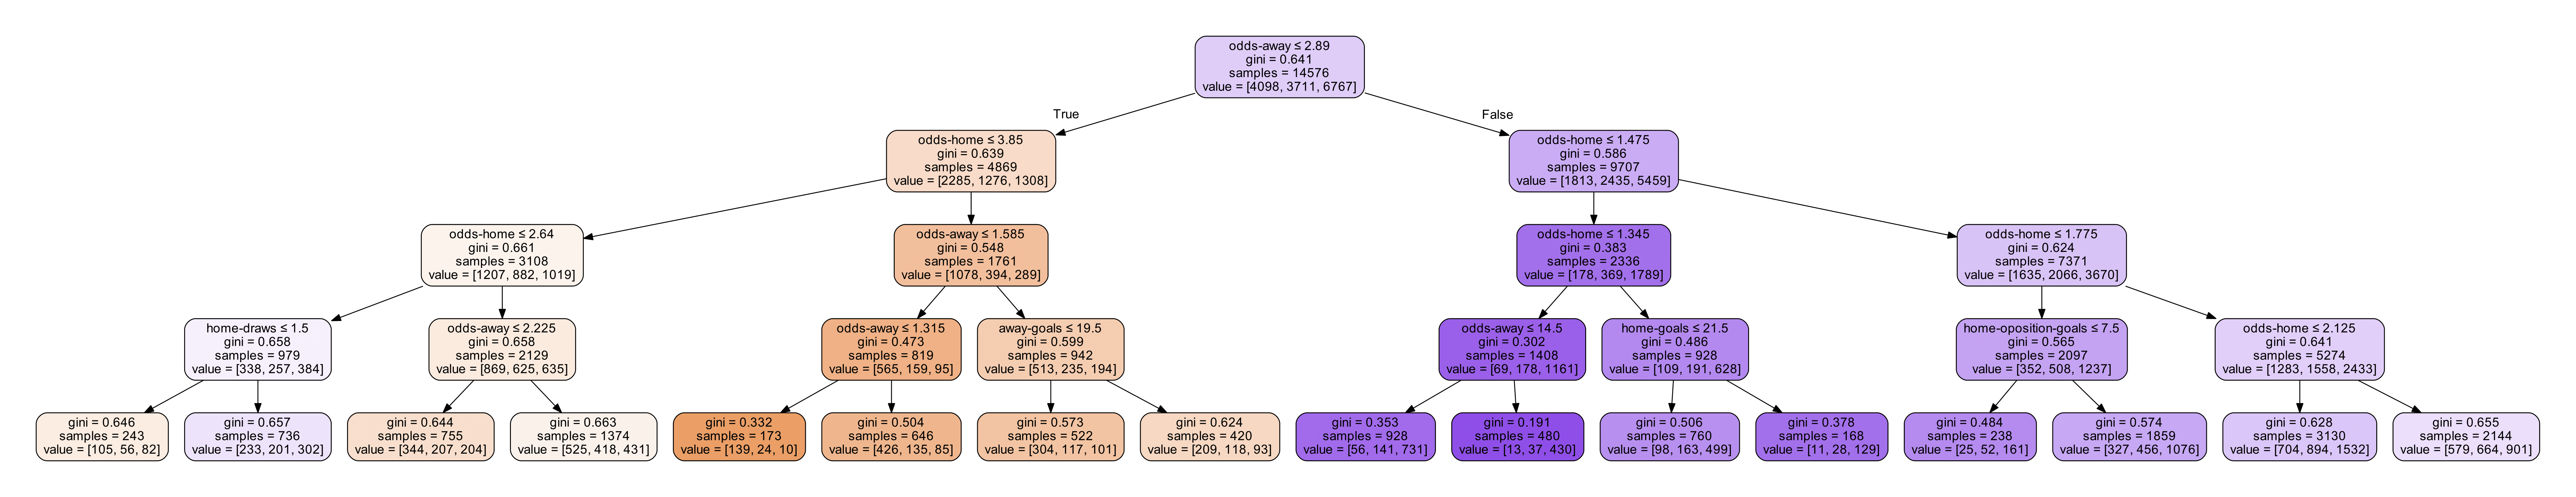
\includegraphics[scale=.075]{DecisionTree.png}
\end{center}
\caption{Decision Tree (max\_depth=4)}
\label{fig:DecisionTree}
\end{figure}


\subsection{Multi-layer Perceptron}

Multi-layer Perceptron (MLP) is a supervised learning algorithm consisting of three layers: one input layer, one hidden layer, and one output layer. The units in the hidden layer are fully connected to the input layer, and the output layer is fully connected to the hidden layer.\newline \newline %\cite{PythonMachineLearning}
In our MLP Model, we used the first sliding window with 13 features in the input layer, two hidden layers, 52 neurons in the first one and 32 neurons in the second one. For the output layer, we have 3 neurons.\newline \newline  
To be able to solve our problem, we used the sigmoid activation function(logistic) for the hidden layers and the softmax activation function for the output layer. We also used a stochastic gradient descent optimizer as a solver. \newline 
As we see in the following plot, the graph of the cost function indicating that the training algorithm converged after the 90th epoch. \newline
\begin{figure}[H]
\begin{center}
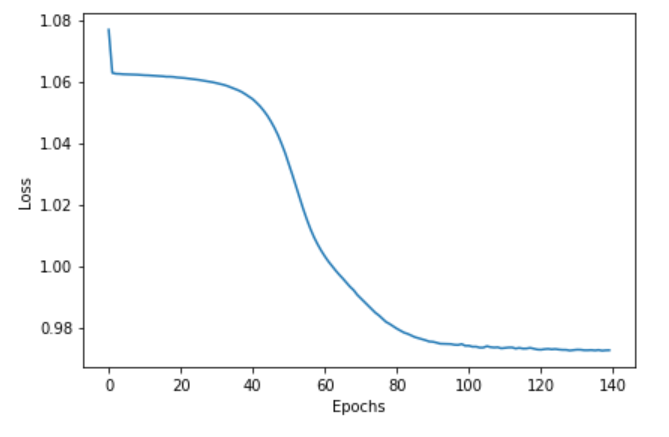
\includegraphics[scale=.7]{MLPcostfunction.png}
\end{center}
\caption{MLP Cost function}
\label{fig:MLPcostfunction}
\end{figure}
The last step is to evaluate the performance of the model by calculating the accuracy of the prediction. We obtained 53.45\% for the training dataset and 52.77\% for the testing dataset.

\subsection{Keras Sequential Neural Network}

To build the model, we used Sequential as a model type. Sequential is the easiest way to create a model in Keras. It allows to build a model layer by layer. Each layer has weights that correspond to the layer that follows it.\newline%\cite{buildingDLModel}
The chosen layer type is 'dense'. Dense is a standard layer type that works for most cases. In a dense layer, all the nodes in the previous layer connect to the nodes in the current one.\newline
As activation function for the hidden layers 'Rectified Linear Activation' (ReLU) was used and 'Softmax' for the output layer. Softmax sums the output up to 1 so that the output can be interpreted as probabilities. The model will then make its prediction according to the option which has a higher probability.\newline \newline
The first layer needs an input shape. The input shape specifies the number of rows and columns in the input.\newline
The last layer is the output layer. It has three nodes - one for each option: Home Win, Draw or Away Win, which is for our prediction, as shown in the following line of codes.\newline \newline
\begin{lstlisting}[language=Python, caption=Python code for simple Keras Sequantial Model Instantiation]
model = tf.keras.Sequential([ 
  layers.Dense(13, activation='relu',input\_shape=(train\_X.shape[1],)), 
  layers.Dense(16, activation='relu'),
  layers.Dense(8, activation='relu'),
  layers.Dense(3, activation='softmax')
])
\end{lstlisting}
To compile the model, we chose Adam as an optimizer. The Adam Optimizer adjusts the learning rate throughout the training.\newline
The learning rate determines the speed at which the optimal weights for the model are calculated.\newline
For the loss function, we chose $sparse\_categorical\_crossentropy$. It is one of the most common choices for classification. A lower score indicates that the model is performing better.\newline \newline
Weight regularization is a regularization technique that provides an approach to reduce over-fitting of a deep learning neural network model on training data and to improve the performance of the model on new data.\newline
By default, no regularizer is used in layers. For this, we made some models with the addition of the L2 regularization, which is the sum of the squared weights.\newline \newline
In other models, we have added dropout, which is another regularization technique for neural networks, to avoid over-fitting in neural networks. Additionally we combined both regularization techniques in one model. \autoref{table:colab_nn} shows the test-accuracies of the models in comparison.

The evolution of the loss-function of the generated models over time can be seen in \autoref{fig:ModelCompare}.

\begin{figure}[H]
\begin{center}
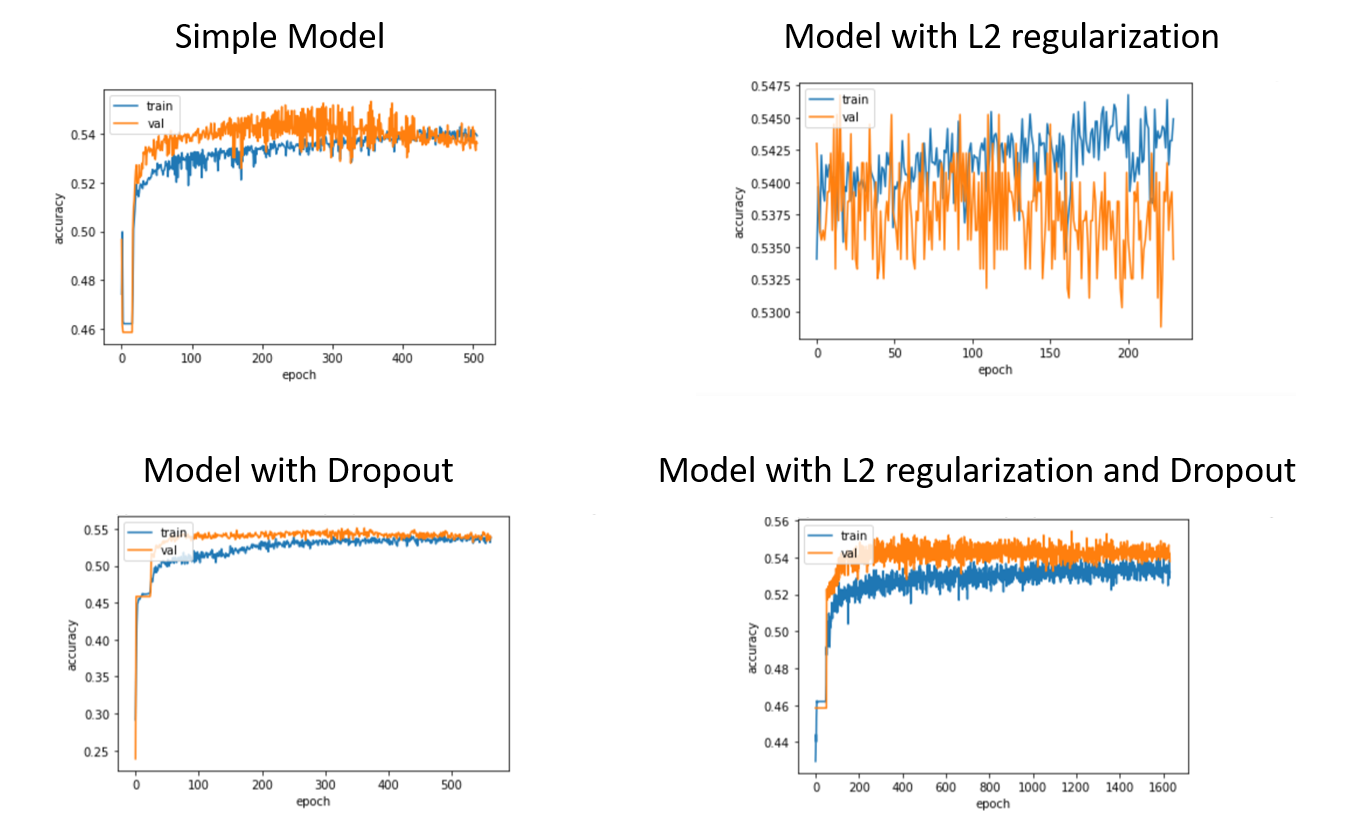
\includegraphics[scale=.6]{ModelCompare.png}
\end{center}
\caption{Evolution of the loss function of the models over time}
\label{fig:ModelCompare}
\end{figure}

\begin{table}
\centering
\label{table:colab_nn}
\begin{tabular}{|p{2cm}|p{2cm}|p{3cm}|p{2cm}|p{3cm}|}
\hline
 & \textbf{Normal} & \textbf{L2-Weight \newline Regularization} & \textbf{Dropout} & \textbf{Dropout \& \newline Regularization} \\ \hline
\textbf{Model01} & 0.5220729 & 0.5191939 & 0.5191939 & 0.5268714 \\ \hline
\textbf{Model02} & 0.5198864 & 0.52272725 & 0.5369318 & 0.50852275 \\ \hline
\textbf{Model03} & 0.4943182 & 0.4971591 & 0.5113636 & 0.50852275 \\ \hline
\textbf{Model04} & 0.5057143 & 0.5114286 & 0.49142858 & 0.4857143 \\ \hline
\textbf{Model05} & 0.5 & 0.49714285 & 0.4942857 & 0.50285715 \\ \hline

\end{tabular}
\caption{Test-accuracy of various models with different parameters}
\label{table:colab_nn}
\end{table}

To get a better feeling for the impact the number of hidden layers and the amount of neurons within each hidden layer have on the overall performance of the model, we conducted a series of tests.\newline
We tested each sliding window option with a varying amount of hidden layers (\textbf{H1}-\textbf{H4}) and a varying number of neurons per layer (\textbf{H}igh, \textbf{M}edium, \textbf{L}ow and \textbf{F}unnel).\newline
The architectures of the neural nets can be found in \autoref{section:appendix_a}.\newline

The test-accuracies for the models based on sliding window option 1 can be seen in \autoref{table:nn_variation_sliding_01}.

\begin{table}
\centering
\begin{tabular}{|l|l|l|l|l|}
\hline

\textbf{Model01} & \textbf{H} & \textbf{M} & \textbf{L} & \textbf{F} \\ \hline
\textbf{H1} & 0.537428 & 0.53358924 & 0.5460653 & - \\ \hline
\textbf{H2} & 0.53262955 & 0.537428 & 0.53454894 & - \\ \hline
\textbf{H3} & 0.5422265 & 0.537428 & 0.47408828 & 0.5393474 \\ \hline
\textbf{H4} & 0.5431862 & 0.5393474 & 0.537428 & 0.537428 \\ \hline

\end{tabular}
\caption{Test-accuracies for variation of hidden layers and neurons for sliding window option 1}
\label{table:nn_variation_sliding_01}
\end{table}

\autoref{table:nn_variation_sliding_02} shows the test-accuracies for the models based on sliding window option 2.

\begin{table}
\centering
\begin{tabular}{|l|l|l|l|l|}
\hline

\textbf{Model02} & \textbf{H} & \textbf{M} & \textbf{L} & \textbf{F} \\ \hline
\textbf{H1} & 0.52840906 & 0.53409094 & 0.52840906 & - \\ \hline
\textbf{H2} & 0.5198864 & 0.5255682 & 0.53125 & - \\ \hline
\textbf{H3} & 0.5255682 & 0.53125 & 0.5369318 & 0.5369318 \\ \hline
\textbf{H4} & 0.5198864 & 0.5198864 & 0.53977275 & 0.5255682 \\ \hline

\end{tabular}
\caption{Test-accuracies for variation of hidden layers and neurons for sliding window option 2}
\label{table:nn_variation_sliding_02}
\end{table}

\autoref{table:nn_variation_sliding_03} shows the test-accuracies for the models based on sliding window option 3.

\begin{table}
\centering
\begin{tabular}{|l|l|l|l|l|}
\hline

\textbf{Model03} & \textbf{H} & \textbf{M} & \textbf{L} & \textbf{F} \\ \hline
\textbf{H1} & 0.53977275 & 0.5426136 & 0.5511364 & - \\ \hline
\textbf{H2} & 0.5625 & 0.5568182 & 0.54545456 & - \\ \hline
\textbf{H3} & 0.53977275 & 0.5369318 & 0.5625 & 0.53977275 \\ \hline
\textbf{H4} & 0.5625 & 0.5426136 & 0.54545456 & 0.5426136 \\ \hline

\end{tabular}
\caption{Test-accuracies for variation of hidden layers and neurons for sliding window option 3}
\label{table:nn_variation_sliding_03}
\end{table}

\autoref{table:nn_variation_sliding_04} shows the test-accuracies for the models based on sliding window option 4.

\begin{table}
\centering
\begin{tabular}{|l|l|l|l|l|}
\hline

\textbf{Model04} & \textbf{H} & \textbf{M} & \textbf{L} & \textbf{F} \\ \hline
\textbf{H1} & 0.5342857 & 0.5342857 & 0.5342857 & - \\ \hline
\textbf{H2} & 0.5257143 & 0.5371429 & 0.5342857 & - \\ \hline
\textbf{H3} & 0.5314286 & 0.5342857 & 0.5314286 & 0.52 \\ \hline
\textbf{H4} & 0.5285714 & 0.5285714 & 0.5285714 & 0.5228571 \\ \hline

\end{tabular}
\caption{Test-accuracies for variation of hidden layers and neurons for sliding window option 4}
\label{table:nn_variation_sliding_04}
\end{table}

\autoref{table:nn_variation_sliding_05} shows the test-accuracies for the models based on sliding window option 5.

\begin{table}
\centering
\begin{tabular}{|l|l|l|l|l|}
\hline

\textbf{Model05} & \textbf{H} & \textbf{M} & \textbf{L} & \textbf{F} \\ \hline
\textbf{H1} & 0.5342857 & 0.52 & 0.5314286 & - \\ \hline
\textbf{H2} & 0.5228571 & 0.5314286 & 0.5371429 & - \\ \hline
\textbf{H3} & 0.5342857 & 0.5228571 & 0.5314286 & 0.5371429 \\ \hline
\textbf{H4} & 0.5228571 & 0.5257143 & 0.5314286 & 0.52 \\ \hline

\end{tabular}
\caption{Test-accuracies for variation of hidden layers and neurons for sliding window option 5}
\label{table:nn_variation_sliding_05}
\end{table}

